\documentclass[problem]{mcs}

\begin{pcomments}
  \pcomment{PS_koch_induction}
  \pcomment{ALGEBRA SHOULD BE CHECKED}
  \pcomment{elaboration of PS_koch_snowflake}
  \pcomment{ARM 4/9/14}
\end{pcomments}

\pkeywords{
  induction
  equilateral
  recurrence
  geometric
  sum
}

%%%%%%%%%%%%%%%%%%%%%%%%%%%%%%%%%%%%%%%%%%%%%%%%%%%%%%%%%%%%%%%%%%%%%
% Problem starts here
%%%%%%%%%%%%%%%%%%%%%%%%%%%%%%%%%%%%%%%%%%%%%%%%%%%%%%%%%%%%%%%%%%%%%

\begin{problem}
Let's define a sequence of polygons $S_0, S_1$ recursively, starting
with $S_0$ equal to a unit square.  We construct $S_{n+1}$ by removing
the middle third of each edge of $S_n$ and replacing it with two line
segments of the same length, as illustrated in Figure~\ref{kochline}.
Let $a_n$ be the area of $S_n$.  So $a_0 =1$ and $a_1$ equals $a_0$
plus the area of four equilateral triangles with side 1/3.  Namely,
\begin{equation}\label{a1141}
a_1 = 1 + 4 \cdot \frac{\sqrt{3}}{4}\paren{\frac{1}{3}}^2 = 1 + \frac{\sqrt{3}}{9}.
\end{equation}

 Prove by induction that for $n>0$,
\begin{equation}\label{an1s3}
  a_n = 1 + \frac{\sqrt{3}}{5} \paren{1 - (4/9)^n}
\end{equation}

\begin{staffnotes}
\hint  If need be, prompt for the recurrence~\eqref{an+1a}.
\end{staffnotes}

\begin{figure}
  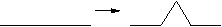
\includegraphics[width=2.5in]{koch}
  \caption{Updating an edge of $S_n$.}
  \label{kochline}
\end{figure}

\begin{solution}
Let $l_n$ be the length of the edges in $S_n$, and $e_n$ be the number
of edges in $S_n$.  So, $l_0=1$, and $e_0=4$.  From the definition of
$S_{n+1}$, we have
\begin{align}
l_{n+1} & = \frac{l_n}{3},\label{ln+13}\\
e_{n+1} & = 4e_n,\label{en+14}\\
a_{n+1} & = a_n + e_n \cdot \frac{\sqrt{3}}{4}\paren{l_{n+1}}^2.\label{an+1a}
\end{align}

Clearly,
\begin{equation}\label{ln/en}
l_n = \paren{\frac{1}{3}}^{n} \qquad \text{and}\qquad e_n = 4^{n+1},
\end{equation}
as can be verified by a trivial induction.

We now use~\eqref{an+1a} to prove by induction on $n$
that~\eqref{an1s3} holds for all $n \geq 1$, with~\eqref{an1s3} serving as
induction hypothesis.

\begin{proof}
\inductioncase{Base case}: ($n=1$). $a_1$ is given in~\eqref{a1141} to which the 
right hand side of~\eqref{an1s3} simplfies when $n=1$.

\inductioncase{Induction step}: \TBA{fill in}

\end{proof}

By the way, we derived~\eqref{an1s3} using the formula for a geometric sum:
\begin{align*}
a_n & =  a_{n-1} + 4^n \cdot\frac{\sqrt{3}}{4} (1/9)^n\\
    & =  a_{n-1} + \frac{\sqrt{3}}{4}(4/9)(4/9)^{n-1}\\
    & = 1 + \frac{\sqrt{3}}{9}\sum_{k=0}^{n-1} \paren{\frac{4}{9}}^k\\
    & = 1 + \frac{\sqrt{3}}{9} \frac{1 - (4/9)^n}{1-4/9}\\
    & = 1+  \frac{\sqrt{3}}{9} \frac{9}{5}\paren{1 - (4/9)^n}\\
    & = 1+  \frac{\sqrt{3}}{5} \paren{1 - (4/9)^n}.
\end{align*}

So as $n$ goes to infinity, the area $a_n$ approaches $1+ \sqrt{3}/5$
while the perimeter approaches a nowhere differentiable curve whose
length is $\lim_{n \to \infty} e_n l_n = \lim_{n \to \infty} (4/3)^n =
\infty$.

\end{solution}

\end{problem}

%%%%%%%%%%%%%%%%%%%%%%%%%%%%%%%%%%%%%%%%%%%%%%%%%%%%%%%%%%%%%%%%%%%%%
% Problem ends here
%%%%%%%%%%%%%%%%%%%%%%%%%%%%%%%%%%%%%%%%%%%%%%%%%%%%%%%%%%%%%%%%%%%%%

\endinput

